\documentclass[border=2mm]{standalone}
\usepackage{pgfplots}
\pgfplotsset{compat=1.18}
\definecolor{red}{rgb}{0.7, 0.11, 0.11}
\definecolor{blue}{rgb}{0.0, 0.20, 0.42}
\definecolor{green}{rgb}{0.11, 0.35, 0.02}
\begin{document}
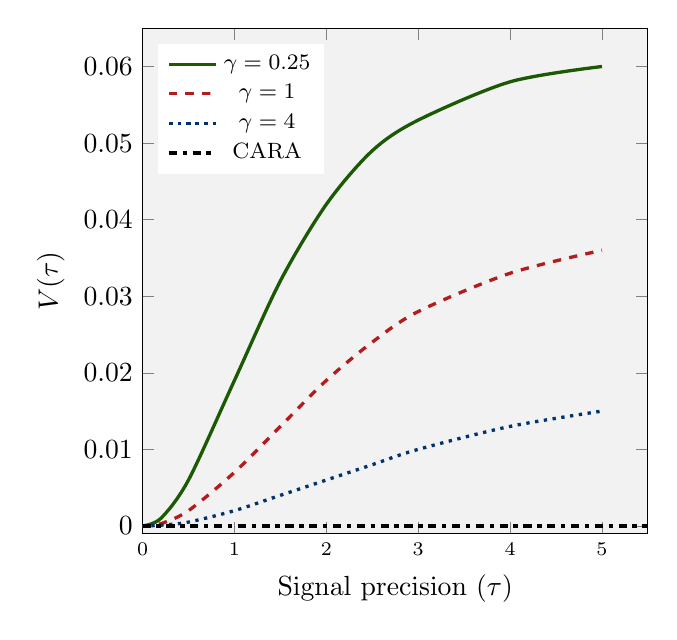
\begin{tikzpicture}
\begin{axis}[
  legend style={draw=none,legend pos=north west,font=\footnotesize},
  ticklabel style={/pgf/number format/fixed,/pgf/number format/precision=5},
  scaled ticks=false,
  ymin=-0.001, ymax=0.065, ylabel={$V(\tau)$},
  xmin=0, xmax=5.5, xlabel={Signal precision ($\tau$)},
  xticklabel style={font=\scriptsize},
  width=8cm, height=8cm,
  axis background/.style={fill=black!5}]

% gamma = 0.25 (invented)
\addplot[very thick,color=green,smooth] coordinates {
  (0,0)(0.2,0.001)(0.5,0.006)(1.0,0.019)(1.5,0.032)
  (2.0,0.042)(2.5,0.049)(3.0,0.053)(4.0,0.058)(5.0,0.060)};

% gamma = 1 (invented)
\addplot[very thick,color=red,dashed,smooth] coordinates {
  (0,0)(0.2,0.0003)(0.5,0.002)(1.0,0.007)(1.5,0.013)
  (2.0,0.019)(2.5,0.024)(3.0,0.028)(4.0,0.033)(5.0,0.036)};

% gamma = 4 (invented)
\addplot[very thick,color=blue,dotted,smooth] coordinates {
  (0,0)(0.2,0.0001)(0.5,0.0005)(1.0,0.002)(1.5,0.004)
  (2.0,0.006)(2.5,0.008)(3.0,0.010)(4.0,0.013)(5.0,0.015)};

% CARA
\addplot[ultra thick,color=black,dashdotted] coordinates {(0,0)(5.5,0)};

\legend{$\gamma = 0.25$, $\gamma = 1$, $\gamma = 4$, CARA}
\end{axis}
\end{tikzpicture}
\end{document}
